% Chapter 2

\chapter{Revisão da Literatura}	%The main chapter title
\label{Chapter2}

Após o capítulo \ref{Chapter1}, onde foi definida a metodologia na secção \ref{sec:metodologia}, agora serão apresentados  e analisados os principais artigos selecionados e as respetivas fontes e autores mais relevantes sobre esta metodologia.
A revisão da literatura pretende primeiramente fazer uma análise bibliométrica e após a mesma,  será feita uma apreciação crítica. Logicamente, que esta revisão de literatura é baseada nos artigos  abaixo indicados e com referências bibliográficas adicionais para completar o estudo.
%1. Pesquisa Bibliográfica (c/ base numa análise bibliométrica c/ mínimo de 30 referências bibliográficas) • Definir a estratégia de pesquisa; • Identificar as bases de dados relevantes; • Definir os critérios de inclusão/exclusão.

%Como funciona: Primeiro apresenta a análise bibliométrica (mapas, gráficos, autores mais citados),
%depois faz uma síntese crítica dos principais artigos (não necessariamente um por seção, mas destacando os 7 mais relevantes dentro dos temas).

%%%%%%%%%%%%%%%%%%%%%%%%%%%%%%%%%%%%%%%%%%%%%%%%%%%%%%%%%%%%%%%%%%%%%%%%%%%%%%%
\section{Análise Bibliométrica}
\label{sec:analise_bibliometrica}

%2. Revisão da Literatura (c/ base numa análise bibliométrica c/ mínimo de 30 referências bibliográficas) • Identificar os principais contributos e seus autores; • Identificar áreas de influência e interesse. Maior ênfase em 7 referências bibliográficas;Peso maior!
A análise bibliométrica aqui presente é um fator crucial para identificar os principais artigos, fontes e autores filtrados de acordo com os artigos escolhidos, esta foi criada em um ficheiro \gls{excel} submetido para avaliação e que está disponível no repositório \gls{github} associado a este relatório \cite{JunqueiraDevEduardoRepositório}.
A revisão da literatura foca-se apenas em 7 artigos selecionados sendo que os restantes 529 artigos serviram apenas para contextualização de mapas no \gls{vosviewer}, como já foi referido pela metodologia na secção \ref{sec:metodologia}.

Assim, esta análise bibliométrica, que integra a revisão de literatura dos 7 artigos selecionados, tem três objetivos principais para identificar os principais indicadores de desempenho \gls{kpi}s dos "\textbf{Artigos}", "\textbf{Fontes}" e "\textbf{Autores}" mais relevantes.

Para tal foram calculados os seguintes indicadores para os "\textbf{Artigos}":
\begin{itemize}
    \item Ano de publicação - com maior ênfase nos últimos 10 anos (2016 a 2026);
    \item Nº de citações nos artigos tendo como base a plataforma do \gls{wos} variando de (17 a 224 citações);
    \item Fontes de publicação mais relevantes com a \gls{query};
    \item Nº de citação do artigo por ano (4 a 32 citações/ano);
    \item Nº de referências no artigo (6 a 155 referências);
    \item Autores mais relevantes (quantidade de vezes que o autor é citado em artigos da sua posse), análise mais estruturada em "\textbf{ Autores }";
    \item Nº de autores em cada artigo (1 a 10) .
    \item \textit{Keywords} do artigo mais relevantes com a \gls{query}.
    \item Interpretação do \textit{"Abstract"} que contemple a \gls{query}.
    \item Países como Portugal, Espanha e Polónia que são filtros de escolha adicionais por Eduardo Junqueira, porque já viveu nas capitais destes 3 países, adquiriu conhecimento prévio real que ajuda na explicação desta temática.
\end{itemize}

Agora os seguintes indicadores para as "\textbf{Fontes}":
\begin{itemize}
    \item Fonte de publicação: (Clean Technologies; Sustainability;\gls{ejor};
Transportation Research Procedia;
International Journal of Logistics Research and Applications;
Energies;
Smart Cities), estão todas relacionadas com a \gls{query};
    \item Nível dos últimos 5 anos de impacto do jornal (3.60 a 6.20);
    \item Categoria do quartil do jornal (Q1 a Q3);
    \item Categoria rank do jornal (14 a 112);
 \end{itemize}

Por fim  os seguintes indicadores para os "\textbf{Autores}":
\begin{itemize}
    \item Nº de publicações do autor na plataforma do \gls{wos} variando de (3 a 303 publicações);
    \item Nº de citações do autor desde sempre na plataforma do \gls{wos} (19 a 4957 citações);
    \item Nº de referências no artigo (6 a 155 referências);
    \item Classificação global do autor no modelo: \gls{hindex} na plataforma do \gls{wos} (1 a 41);
\end{itemize}
\newpage
%%%%%%%%%%%%%%%%%%%%%%%%%%%%%%%%%%%%%%%%%%%%%%%%%%%%%%%%%%%%%%%%%%%%%%%%%%%%%%%%

%3. Análise bibliométrica + síntese crítica dos principais artigos (7 referências bibliográficas) • Apresentar mapas, gráficos, autores mais citados; • Destacar os principais contributos e limitações de cada artigo.
\section{Apreciação Crítica dos Principais Artigos}
\label{sec:apreciacao_critica_principais_artigos}

Nesta secção serão apresentados os 7 artigos desde a sua análise crítica até os principais contributos e limitações de cada um.

Dos 536 artigos fornecidos pelo \gls{wos} através da filtragem feita anteriormente definida pela metodologia na secção \ref{sec:metodologia} e agora pela análise bibliométrica, foram destacados os seguintes:
\textbf{Artigo I:}  "A Review of Technical Standards for Smart Cities"\cite{article}.
\textbf{Artigo II:} "AI-Driven Optimization of Urban Logistics in Smart Cities: Integrating Autonomous Vehicles and IoT for Efficient Delivery Systems"\cite{su162411265}.
\textbf{Artigo III:} "Collaborative urban transportation: Recent advances in theory and practice"\cite{CLEOPHAS2019801}.
\textbf{Artigo IV:} "Shortening the Last Mile in Urban Areas: Optimizing a Smart Logistics Concept for E-Grocery Operations"\cite{article2}.
\textbf{Artigo V:} "Designing new models for energy efficiency in urban freight transport for smart cities and its application to the Spanish case"\cite{NAVARRO2016314}.
\textbf{Artigo VI:} "Fulfilment of last-mile urban logistics for sustainable and inclusive smart cities: a case study conducted in Portugal"\cite{Correia02062024}.
\textbf{Artigo VII:} "Interaction with City Logistics Stakeholders as a Factor of the Development of Polish Cities on the Way to Becoming Smart Cities"\cite{en15114103}.


\textbf{De notar que:} esta escolha de artigos não foi aleatória como é lógico, mas não seguiu uma regra específica de máximo de citações ou melhor autor, ou outro fator, mas sim os melhores de acordo com todos estes indicadores e somente os artigos  do tipo: \textit{open-access} (acesso livre) na plataforma do \gls{wos}.

Para uma ilustração mais clara e sucinta do que será abordado, abaixo a seguinte \gls{fig} \ref{fig:analiseArtigos} realizada na ferramenta \textit{infographic Notebook KLM} da \textit{Microsoft}, ilustra de forma resumida os principais pontos de cada artigo selecionado \cite{JunqueiraDevEduardoNoteBookKLM}.
\begin{figure}[H]
    \centering
    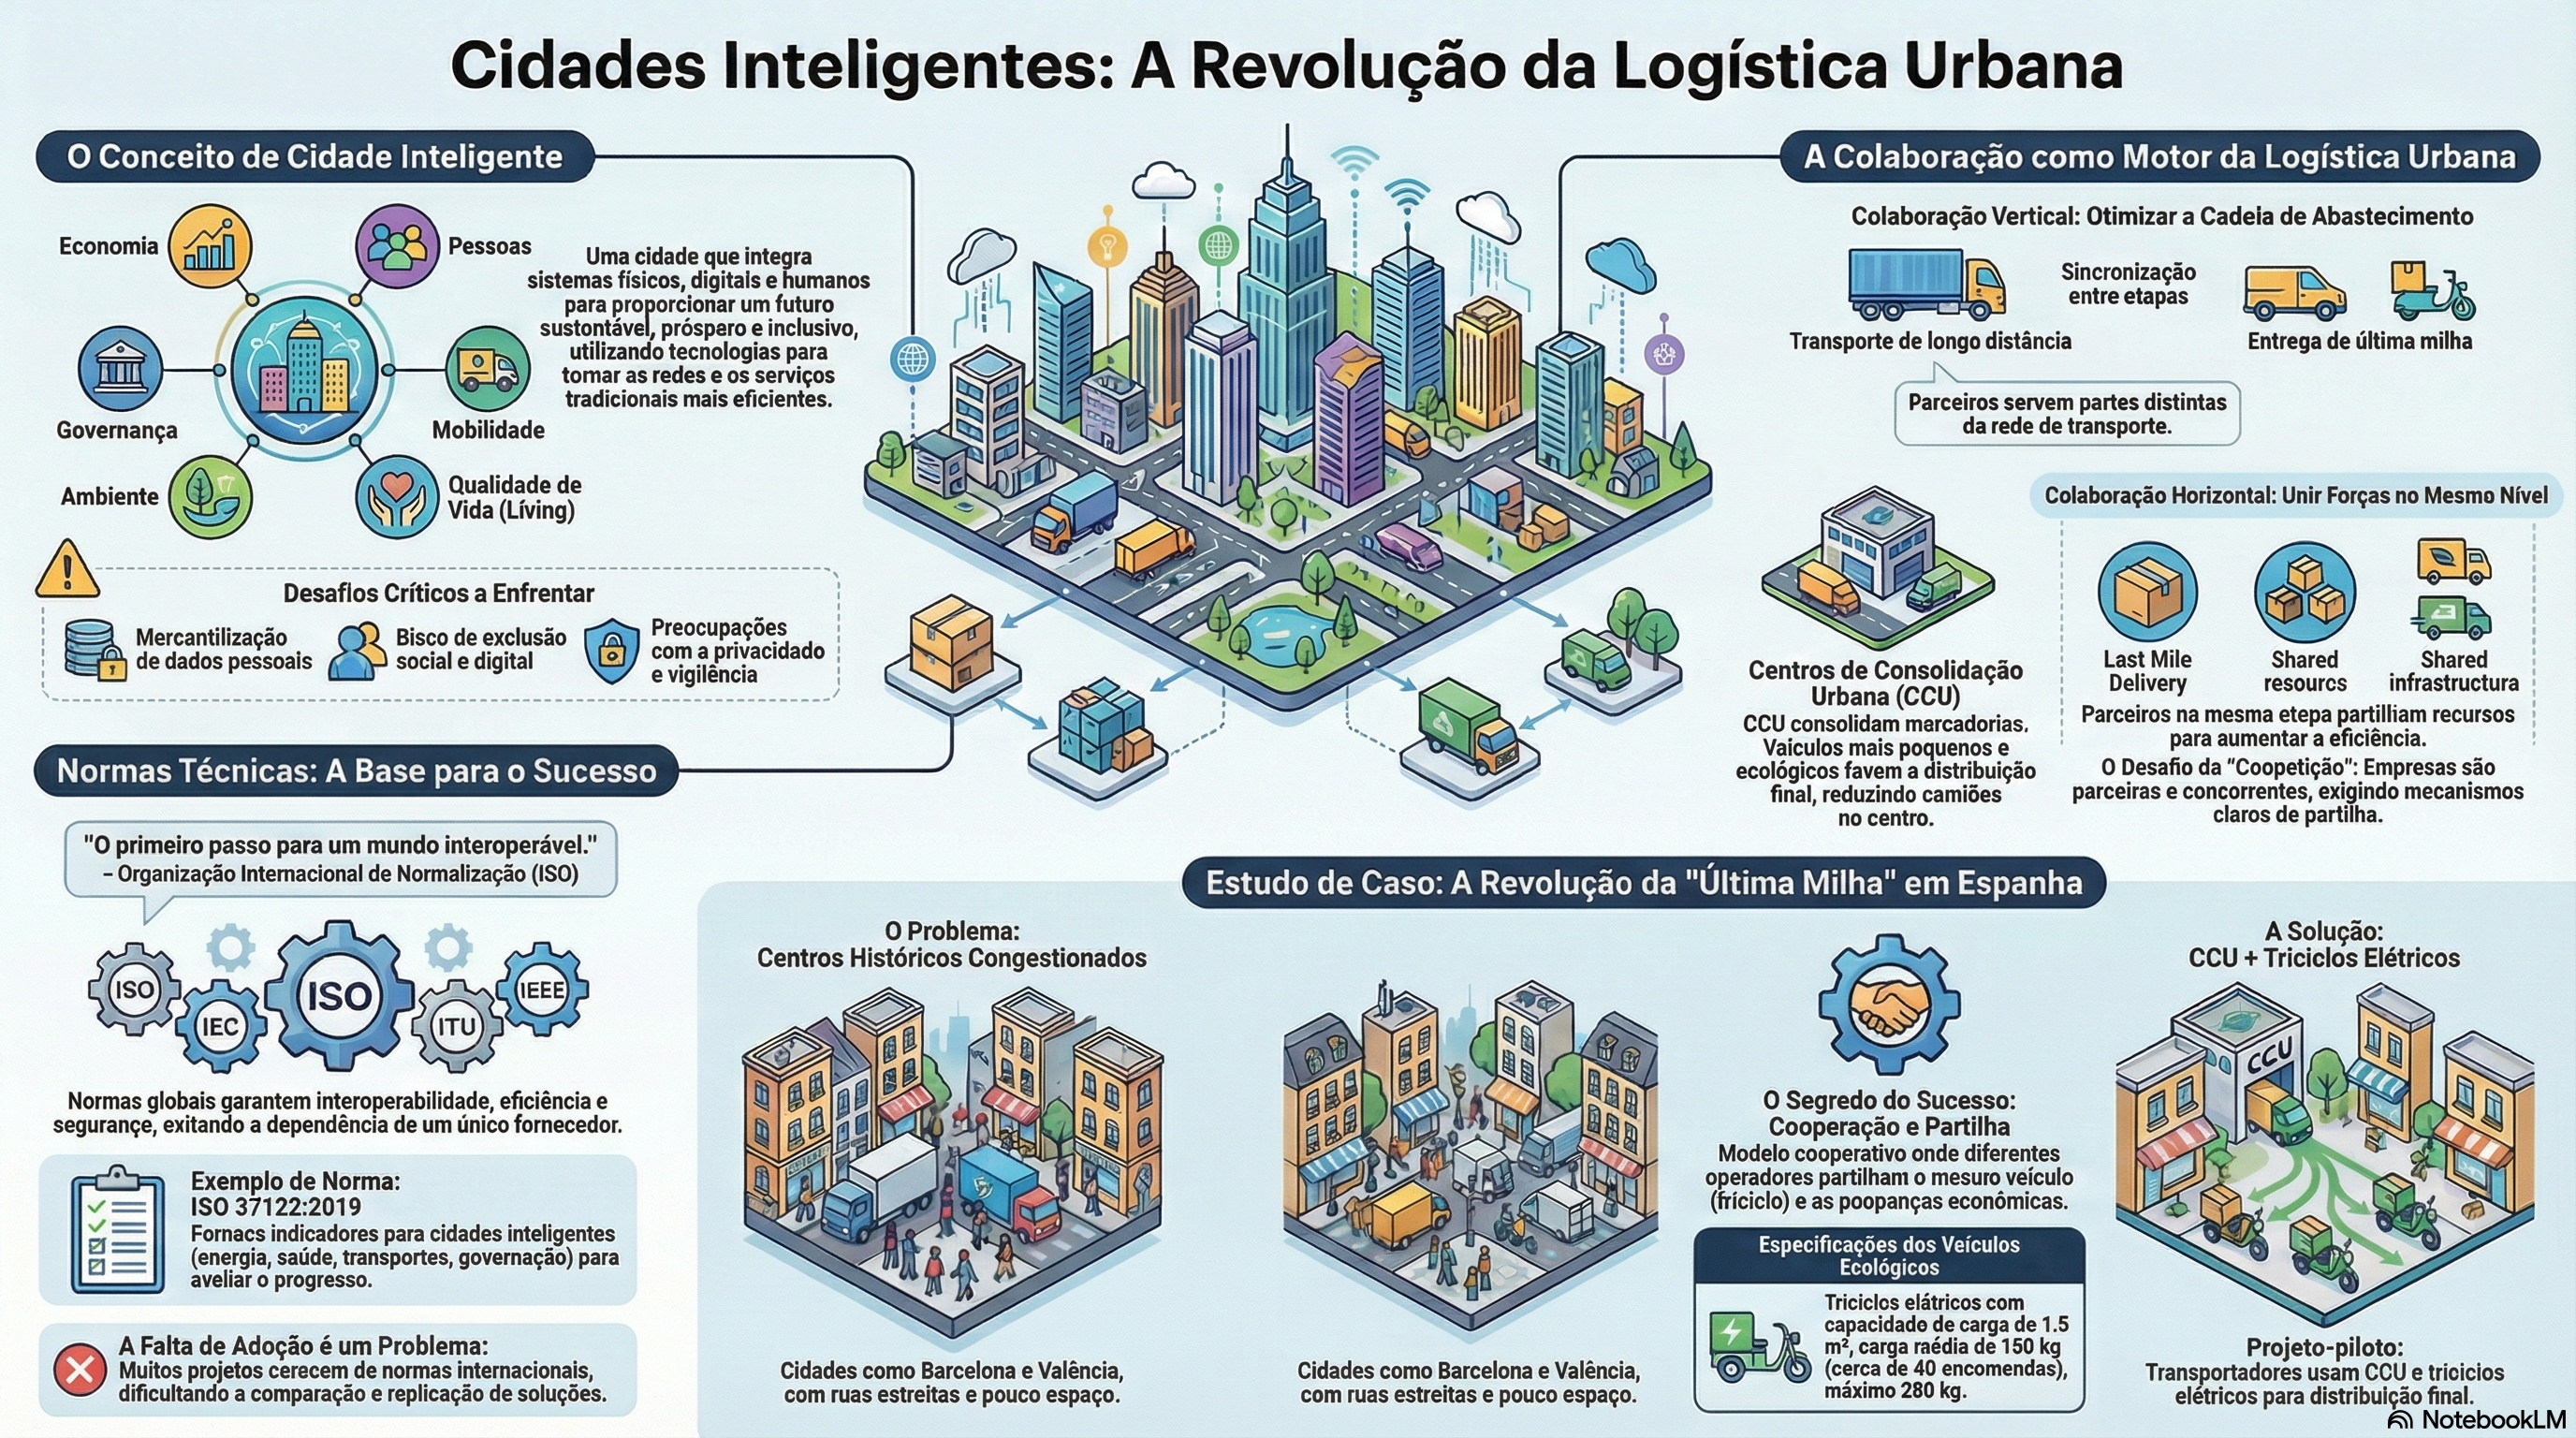
\includegraphics[width=1.1\textwidth]{figures/LKM/review_all.png}
    \caption{Gráfico de comunicação de dados entre normas, conceitos, colaboração e estudo de caso, ferramenta online \textit{infographic Notebook KLM}\cite{JunqueiraDevEduardoNoteBookKLM}.}
    \label{fig:analiseArtigos}
\end{figure}

Uma logística urbana inteligente e eficiente é crucial para uma cidade.
Existe problemas que são comuns com todos os artigos selecionados em relação a este estudo, tais como:
\begin{itemize}
    \item A falta de uma linguagem comum com todos os \textit{stakeholders} envolvidos e clientes finais, ou seja, falta de implementação de um conjunto de normas/regras/padrões globais que todos os países/cidades possam seguir \cite{Correia02062024};
    \item A existência de normas e projetos-piloto que não são aplicados ou replicados em larga escala em casos reais \cite{article};
    \item A falta de integração entre as tecnologias emergentes que estão a ser desenvolvidas \cite{su162411265};
    \item A resistência a mudanças por parte dos operadores logísticos tradicionais e dos clientes finais \cite{en15114103};
    \item A necessidade de fatores publícos e privados trabalharem em conjunto para alcançar soluções eficazes \cite{article};
    \item Contratempos que prejudicam esta integração, tais como: \textit{covid-19}, crises económicas, guerras, taxas de inflação elevadas, entre outros.
\end{itemize}
%%%%%%%%%%%%%%%%%%%%%%%%%%%%%%%%%%%%%%%%%%%%%%%%%%%%%%%%%%%%%%%%%%%%%%%%%%%%%%%%%
\section{Normas Globais para Cidades Inteligentes e Sustentáveis}
\label{sec:normas_globais_cidades_inteligentes_sustentaveis}
Por outro lado, existem contributos importantes a destacar em relação a este estudo.
Uma cidade inteligente não tem um significado único, mas podemos defini-la como uma cidade que usa tecnologia e dados para ter soluções mais informadas. O objetivo é construir um ciclo combinatório para diferentes serviços tais como: os transportes, a eletricidade, a água, o combustível, o lixo,  entre outros, funcionarem em conjunto e não isolados, sendo que o objetivo final é melhorar a qualidade de vida da população urbana.
Cada vez mais as cidades urbanas, cujo o nível de população aumenta de forma exponencial, existe uma tendência crescente de viver em zonas urbanas e deixar as zonas rurais, está previsto que até 2050 cerca de 66\% da população mundial viva em áreas urbanas \cite{article}.

De acordo  com a \gls{iec} a sua missão é o uso mundial das normas Internacionais da \gls{iec} e dos sistemas de avaliação da conformidade para garantir a segurança, eficiência, confiabilidade, integridade e  interoperabilidade das tecnologias elétricas, eletrônicas e da informação, para impulsionar o comércio internacional, facilitar amplo acesso à eletricidade e possibilitar um mundo mais sustentável \cite{IEC}.
A gestão de energia é um dos fatores importante para cidades sustentáveis, como por exemplo o aluguer de painéis solares para edifícios residênciais e comerciais, reduzia o consumo de energia elétrica da rede pública, e aumentaria a energia renovável que é produzida localmente \cite{EnergiaSolar}.
A gestão de água a nível mundial, que existe em abudância por outro lado, logo o desperdício de 3.3 bilhões de litros de água por dia nos países de Inglaterra e País de Gales \cite{article}.
A utilização de dispositivos inteligentes como atuadores e sensores, ou seja produtos, \gls{iot} nem sempre ajuda a reduzir este desperdício, mas sim a serem inteligentes e verificar a quantidade de desperdício, logo se nomeia este processo de \textit{smart water}\cite{article}.

Para garantir estes exemplos, de sustentabilidade de muitos outros, de acordo com o Artigo I, as cidades urbanas devêm ter 6 domínios nomeados de \textit{"Smart"} \cite{article}:
\begin{itemize}
\item \textbf{\textit{Smart economy}}:  Consiste em agrupar a competividade económica que as empressas possuem melhorando a logística de mercados globais entre taxas de produtos ou serviços, entre outros.
\item \textbf{\textit{Smart people}}:  Integração social  é um fator-chave para os clientes finais aceitarem novas soluções e as adotarem de forma eficaz e sustentável. A qualidade da educação e interações sociais são fatores cruciais.
\item \textbf{\textit{Smart governance}}: Normas técnicas globais, devem ser adotadas pelo governo dos países para garantir que os países/cidades, possam se comunicar e trabalhar em conjunto de forma natural. Transparência total de gastos públicos para que as pessoas confiem nas decisões governamentais \cite{article}.
\item \textbf{\textit{Smart mobility}}: Sincronização dos vários meios de transporte públicos tais como metros, comboios, autocarros, bicicletas entre outros e adoção de transportes elétricos e inteligêntes nomeados por \gls{va} \cite{CLEOPHAS2019801}.
\item \textbf{\textit{Smart environment}}: Automatização de sistemas para reduzir o desperdício de recursos naturais, como energia, água, lixo, entre outros \cite{su162411265}.
\item \textbf{\textit{Smart living}}: Qualidade de habitação, segurança, cultura, saúde entre outros fatores que tornam as cidades urbanas mais atrativas para viver.
\end{itemize}

As normas são o centro de tudo, sem estas, estaríamos num processo de \textit{vendor lock-in}, ou seja, cada empresa desenvolveria a sua própria tecnologia/aplicação sem se preocupar com a comunicação entre elas e o consumidor final estaria dependente dessa.
Um exemplo claro é os produtos da \textit{Apple}, a empresa desenvolve um ecossistema de produtos fechado onde para obter o máximo de experiência possível é necessário adquirir todos os produtos do sistema operativo \textit{Apple}, em computadores com processadores unicamente \textit{Apple Silicon}, a utilização de software  fora deste ecossistema é não aconsellhável e muitas vezes impossível de usar.

Portanto, as cidades aqui não devem implementar as suas próprias normas, mais sim de organizações muito relevantes a nível global como \gls{ieee}, \gls{iso}, \gls{itu} e \gls{iec} \textit{International Electrotechnical Commission}  entre outras \cite{article}.
Cada vez mais existe projetos de inovação que tentam implementar estas normas, nomeados de projetos-piloto, uns obtem sucesso, outros não, mas são projetados apenas para um local isolado região urbana, e não replicados por todo o país.

\textbf{De notar que:} certificação, auditoria e gestão de implementação deve acompanhar as normas para evitar incompatibilidades ou falhas no sistema no que diz respeito á comunicação entre diferentes tecnologias \cite{article}.
%%%%%%%%%%%%%%%%%%%%%%%%%%%%%%%%%%%%%%%%%%%%%%%%%%%%%%%%%%%%%%%%%%%%%%%%%%%%%%%%
\section{Papel da \gls{ai} na Logística}
\label{sec:papel_ai_logistica}
A \gls{ai} \textit{Artificial Intelligence}, tem um papel crucial na otimização da logística, permite analisar dados em tempo real, prever padrões específicos, resolver problemas complexos, e automatizar processos. O artigo II relata de uma forma detalhada estes fatores \cite{su162411265}.

A \gls{ai} é uma realidade em construção a ser testada e melhorada em todos os países do mundo. Esta está presente em \gls{iot}, \gls{bigdata}, \gls{ml}, \gls{dl}, \gls{5g} e \gls{va} \textit{Autonomous Vehicle} entre outras tecnologias emergentes \cite{su162411265}.
A recolha de dados em tempo real é realizada por sensores  e atuadores, mas estes precissam de um cérebro central que processe estes dados logo a \gls{ai} está em constante implementação nestas tecnologias.

Existe um modelo de 4 camadas implementado no artigo II  que ajuda a compreender melhor este processo\cite{su162411265}:
\begin{itemize}
    \item \textbf{Camada 1 - Recolha de dados }: Sensores \gls{iot}, dispositivos móveis, câmeras, entre outros recolhem dados em tempo real;
    \item \textbf{Camada 2 - Processamento e \gls{ai} }:  Camada intermédia e a mais importante, os dados brutos recolhidos são limpos e processados pela \gls{ai}.
    \item \textbf{Camada 3 - Controlo}: O sistema toma decisões baseados nos dados processados.
    \item \textbf{Camada 4 - Aplicação}: Visualização final, as decisões são implementadas em operações logísticas reais em interface humana, existe supervisionamento e intervensão humana quando necessário.
\end{itemize}

Contudo, existe desafios ainda não ultrapassados nesta área da \gls{ai} que são: \textbf{I:} A responsabilidade ética caso a \gls{ai} falhe; \textbf{II:} A privacidade dos dados recolhidos até que ponto estes dados são seguros dentro do sistema da \gls{ai}; \textbf{III:} A aceitação por parte dos clientes finais \cite{su162411265}.

\textbf{De notar que:} a eficácia da \gls{ai} na logística depende não apenas da tecnologia, mas também da integração com políticas públicas e da confiança das empressas e clientes finais.
%%%%%%%%%%%%%%%%%%%%%%%%%%%%%%%%%%%%%%%%%%%%%%%%%%%%%%%%%%%%%%%%%%%%%%%%%%%%%%%%
\section{Transporte Colaborativo Urbano}
\label{sec:transporte_colaborativo_urbano}

O congestionamento urbano de transporte é também um fator crucial a ser resolvido, o artigo III  aborda este tema de uma forma detalhada \cite{CLEOPHAS2019801}.
A congestão de trânsito causa: atrasos, emissões de gases poluentes, acidentes, discussões e stress entre condutores, entre outros fatores negativos.
Este transito é proveniente de vários fatores tais como: aumento do número de veículos, falta de transporte público eficiente, aumento de encomendas de transportadoras entre outros \cite{CLEOPHAS2019801}.
Em paíse como a Polónia, Espanha e Portugal, o transporte "carro individual" é o meio de transporte mais utilizado, o que aumenta ainda mais o congestionamento urbano \cite{en15114103, NAVARRO2016314, Correia02062024}.

Existe duas vertentes para resolver este problema de congestionamento de acordo com o artigo III \cite{CLEOPHAS2019801}:
\begin{itemize}
    \item \textbf{Colaboração vertical}: Colaboração entre diferentes níveis da logística de transporte entre fabricantes de produtos, lojas de produtos e transportadoras de produtos, onde todos partilham dados de entregas para melhorar as rotas e reduzir o número de veículos em circulação.
    \item \textbf{Colaboração horizontal}: Colaboração entre empresas da mesma logística de transporte, como por exemplo transportadoras de produtos ou de encomendas podem partilhar dados de entregas para melhorar as rotas e reduzir o número de veículos em circulação.
\end{itemize}

Um exemplo prático da colaboração vertical foi uma cidade costeira no sudoeste da França La Rochelle, que é a capital do departamento de "Charentes-Maritime".
Esta cidade francesa é um importante centro logístico na Europa e é um dos principais destinos para o transporte marítimo de mercadorias na Península Ibérica \cite{FreighttransporttoLaRochelle}.
Esta cidade implementou uma logística de transporte de mercadorias em transportes públicos, ou seja, em entregas nomeadas de \textit{last-mile}, encomendas de diferentes empressas partilham informação logística para envio em transportes públicos levando passageiros e mercadorias em transportes rodoviários, ferroviários, entre outros diminuindo o número de transportadoras (camiões grandes que ocupam espaço muito considerável em uma fila de trânsito) \cite{CLEOPHAS2019801}.

\textbf{De notar que:} sem incentivos contínuos e regras de partilha de custos e ganhos, a colaboração tende a subótimos de baixo rendimento económico \cite{CLEOPHAS2019801}.
%%%%%%%%%%%%%%%%%%%%%%%%%%%%%%%%%%%%%%%%%%%%%%%%%%%%%%%%%%%%%%%%%%%%%%%%%%%%%%%%%%%%
\section{E-Grocery Conceito Logístico de transporte}
\label{sec:egcconceitologisticotransporte}


A urbanização e o crescimento do \textit{e-commerce} e de \gls{egc} aumentam o tráfego e as emissões nas cidades urbanas, são outros fatores em ter em consideração abordados no artigo IV \cite{article2}.
Para mitigar o aquecimento global, a \gls{ue} estabeleceu metas ambiciosas para reduzir gases de efeito estufa.
Até 2030: logística urbana nas principais cidades deve ser praticamente livre de \gls{co2} e até 2050 eliminar veículos movidos por combustíveis fósseis (gasolina e diesel) das cidades \cite{article2}.

Atualmente, existe um aumento exponencial de encomendas de produtos de supermercado em \gls{egc}, devido a vários fatores tais como: pandemia \textit{covid-19}, falta de tempo, comodidade, facilidade de escolha e resposta rápida, entre outros.
Este transporte é feito em veículos pequenos que são mais ágeis no trânsito urbano como por exemplo bicicletas, motociclos, veículos a combustão/elétricos pequenos, mas o número de veículos têm aumentado exponencialmente, causando mais congestionamento urbano \cite{article2}.

Na China, o mercado de \gls{egc} cresceu 23 vezes entre 2013 e 2019, atingindo um valor de 50 mil milhões de dólares em 2019\cite{article2}.
A Alemanha prôpos um sistema de transporte inovador de \textit{last-mile}.
A criação de centro logístico fora da cidade chamados de \textit{Urban Logistics Hub}, como um cacifo grande que armazena encomendas e as restribui para cacifos mais pequenos na cidade, é uma solução para este problema, as encomendas de ultima milha são entregues por estafetas em bicicletas elétricas nomeadas por \gls{bce}  que são mais ágeis no trânsito urbano e não emitem gases poluentes. \cite{article2}.
Este sistema foi testado em 2020 na cidade de Hanover, Alemanha, com resultados positivos e tem como algoritmo a otimização de rotas para as \gls{bce}.

As principais vantagens deste sistema em relação ao convencional por entregas de \textit{Van} carrinha de transporte convencional são: redução de emissões de \gls{co2}, redução de \verb|km/dia| percorrido, e melhor cooredenação entre o consumidor final e as mercadorias\cite{article2}.

As desvantagens deste sistema é o preço elevado de implementação do \textit{Urban Logistics Hub} e o custo associado por dia ao mesmo, dependendo do fator de deslocamento  \verb|km/dia| depende da quantidade de pessoas que utilizarão este sistema a longo prazo.

A \gls{fig} abaixo \ref{fig:egc_conceito_logistico_transporte} ilustra este conceito logístico de transporte na cidade urbana consoante fatores de deslocamentos associados a distâncias mais convenientes para existir uma otimização de rotas mais curtas \gls{egc}.
\begin{figure}[H]
    \centering
    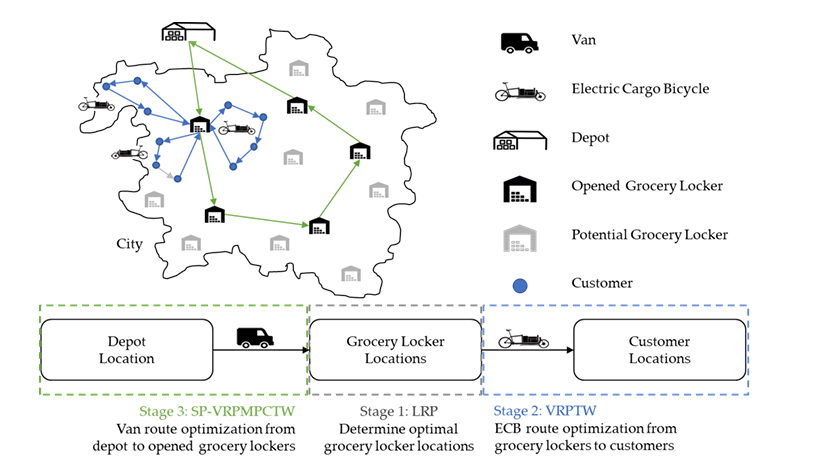
\includegraphics[width=1.25\textwidth]{figures/Artigo4-metodologia-entregas-cacifo.png}
    \caption{Conceito logístico de transporte de \gls{egc}, adaptado na cidade de Hanover, Alemanha citado neste artigo: \cite{article2}.}
    \label{fig:egc_conceito_logistico_transporte}
\end{figure}

Por fim, este conceito logístico de transporte de \gls{egc} é uma solução inovadora para o problema do congestionamento urbano, mas é de notar que a sua implementação apenas benificia o comportamento da empresa que terá menos custos operacionais e não o cliente final que paga o mesmo preço por uma entrega mais sustentável.

\textbf{De notar que:} a experiência do utilizador final pode ser comprometida sem interfaces digitais intuitivas \gls{api}, que permitam rastreamento em tempo real, gestão flexível de horários e ganhos monetários ou outras vantagens que incentivem a adoção deste sistema \cite{article2}.
%%%%%%%%%%%%%%%%%%%%%%%%%%%%%%%%%%%%%%%%%%%%%%%%%%%%%%%%%%%%%%%%%%%%%%%%%%%%%%%
\section {Novos Modelos de Eficiência Energética no Transporte}
\label{sec:novos_modelos_eficiencia_energetica_transporte}
O artigo V, aborda novos modelos de eficiência energética no transporte de mercadorias em cidades inteligentes \cite{NAVARRO2016314}.
O setor rodoviário é um dos maiores contribuintes para as emissões de gases de efeito estufa na \gls{ue}, representando cerca de 20\% do total de CO2. Em áreas urbanas, essa proporção pode chegar a 30\%, devido ao tráfego intenso e às entregas de mercadorias \cite{NAVARRO2016314}.
Para mitigar este problema, é necessário implementar novos modelos de eficiência energética no transporte de mercadorias.

Neste contexto, seis cidades mediterrânicas (Pireu, Bolonha, Montpellier, Rijeka, Barcelona e Valência) colaboraram com o objetivo de contribuir para a melhoria da eficiência energética no transporte urbano de mercadorias como parte do projeto criado em 2015 nomeado de \gls{smile} co-financiado  pela \gls{ue}  \cite{NAVARRO2016314}.
Um dos objetivos em cidades urbanas é preservar o património histórico e cultural, não só para os habitantes locais, mas para os turistas como por exemplo a cidade de Valência em Espanha que é um centro histórico relevante na \gls{ue}.
Este projeto foi replicado e como exemplo em Espanha na cidade de Valência: entregas de última milha com triciclos elétricos assistidos e microplataformas de distribuição entre outubro de 2014 e janeiro de 2015, com resultados positivos\cite{FundacionValenciaport_2020} .

A \gls{fig}: \ref{fig:smilemodeloeficienciaenergetica},  abaixo cita perfeitamente este  novo modelo de eficiência  \gls{smile} no transporte de mercadorias em cidades inteligentes.
\begin{figure}[H]
    \centering
    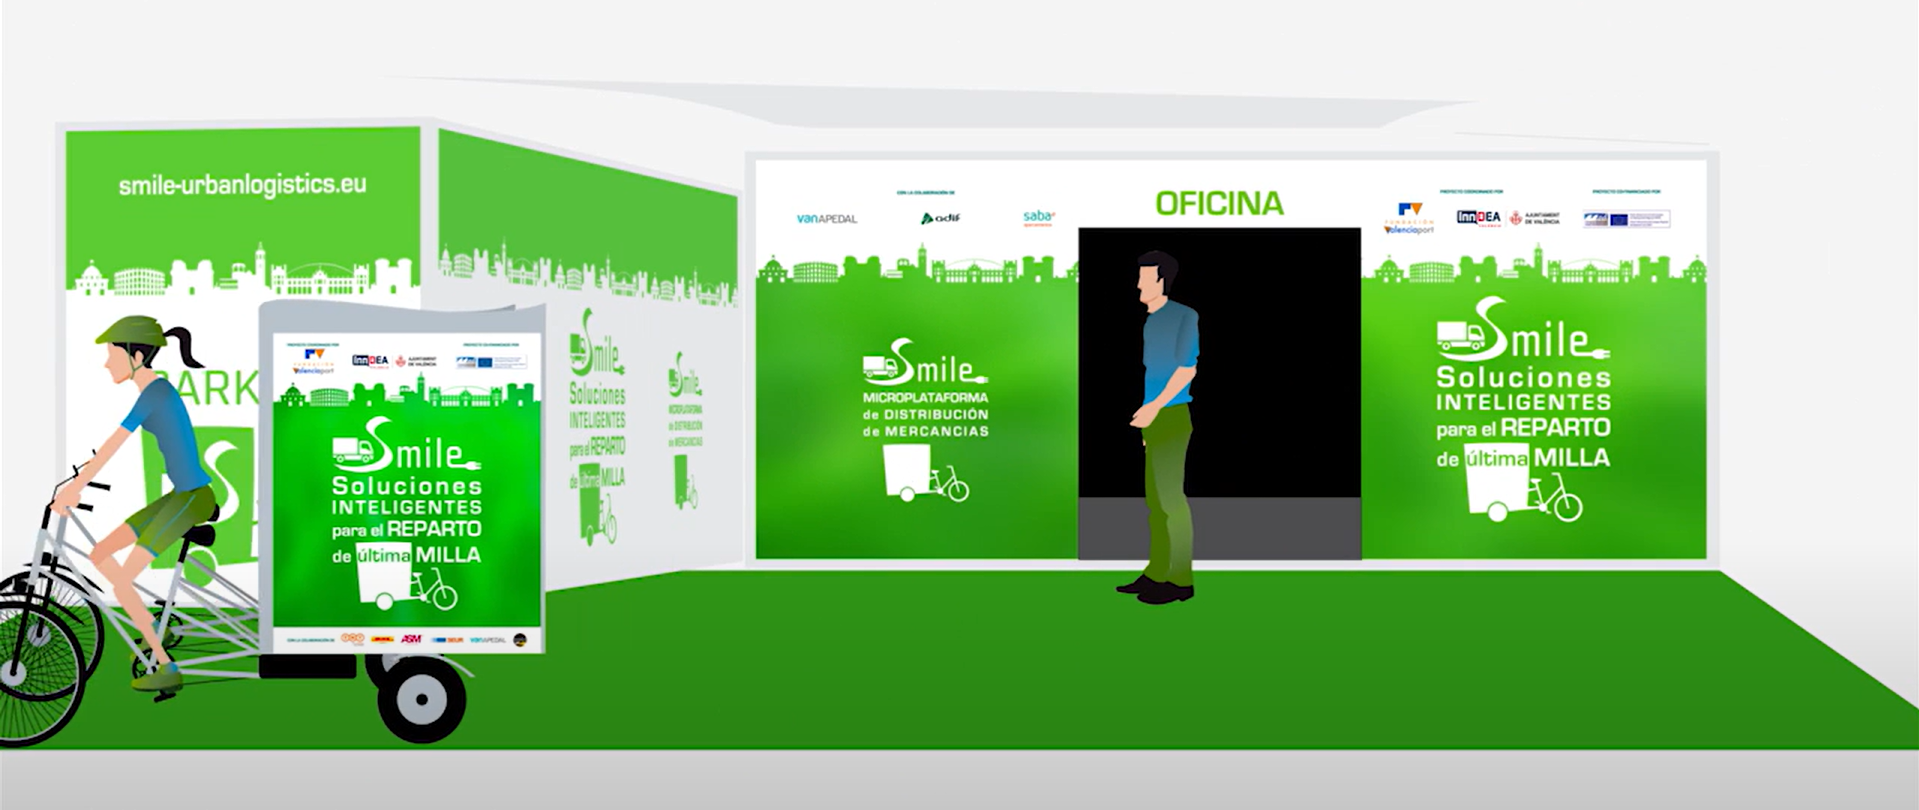
\includegraphics[width=1.25\textwidth]{figures/smile.png}
    \caption{Novo modelo de eficiência energética no transporte de mercadorias em cidades inteligentes citado no vídeo do \gls{smile}: \cite{FundacionValenciaport2015}.}
    \label{fig:smilemodeloeficienciaenergetica}
\end{figure}

\textbf{De notar que:} este artigo V segue o mesmo conceito do artigo IV, mas foca-se mais em eficiência energética no transporte de qualquer encomenda, do que no conceito logístico de transporte comparativo ao tradicional.
Contudo a esta eficiência energética no transporte em ambos os artigos IV e V,  é um fator a ser considerado para uma possível análise comparativa futura para saber qual é o adequado a cada cidade urbana pois todas as cidades têm a sua cultura e história e são todas diferentes, logo a escabilidade destes projetos deve ser analisada consoante cada cidade a implementar \cite{article2, NAVARRO2016314}.
%%%%%%%%%%%%%%%%%%%%%%%%%%%%%%%%%%%%%%%%%%%%%%%%%%%%%%%%%%%%%%%%%%%%%%%%%%%%%
\section{Portugal: Sustentável e Inclusivo}
\label{sec:portugal_sustentavel_inclusivas_cidades_inteligentes
}
O artigo VI, apresenta um estudo muito detalhado,  realizado em Portugal sobre a implementação de soluções logísticas  sustentáveis e inclusivas em cidades urbanas \cite{Correia02062024}.

O principal problema em Portugal é a falta de recursos humanos especializados em logística urbana, coordenação entre empressas públicas, privadas e Municípios (94\% de todos os Munícipios do país, não são capazes de implementar esta logística de forma autónoma, necessitam de cooperação), a falta de ferramentas inovadoras que advém de  estudos em  projeto-pilotos não é aprovada pelos Municípios \cite{Correia02062024}.
As questões ambientais são um fator importante que os Munícipios consideram, mas a falta de recursos financeiros e vontade de mudança são obstáculos que impedem a implementação destas soluções.

\newpage
O estudo  foca-se em um algoritmo de 4 passos para organizar a logística urbana na última milha, com base em dados e colaboração entre \textit{stakeholders} \cite{Correia02062024}:
\begin{itemize}
    \item \textbf{1-Análise de dados históricos:} prevê e procura pontos de mapa com maior densidade de entregas, usa os dados passados para prever os dados futuros;
    \item  \textbf{2-Definir regiões :} Agrupar as regiões de entrega com base em dados históricos através do uso de \textit{clustering} em \textit{data mining}, através de algoritmo como o \gls{dbscan};
    \item  \textbf{3-Conjunto de regiões:} Agrupar as regiões de entrega em conjuntos de regiões com base na proximidade geográfica e volume de entregas, para otimizar as rotas de entrega como modelos especificos de \textit{clustering};
    \item \textbf{4-Localizar os pontos de armazenamento:} Considerando o meio de transporte bicicleta os pontos de armazernamento devem estar localizados em áreas de fácil acesso no centro de cidades num máximo de tempo de 15 minutos, como por exemplo em grandes centros comerciais ou em centros de condomínio residênciais.
\end{itemize}

A opinião dos \textit{stakeholders} foi recolhida através de entrevistas e questionários aplicados a diferentes autárquicos envolvidos no Município urbano.

\textbf{De notar que:} a implementação prática nos Munícipios em cidades inteligentes, exige plataformas colaborativas que permitam partilha segura de dados entre municípios, operadores privados e entidades reguladoras públicas que operam em conjunto, condicionado a  restrições orçamentais, licenciamento urbano e incentivos \gls{ue} \cite{Portugal2030_2023}.

O Município de Águeda é um dos exemplos que adotou o serviço \textit{beÁgueda}. "Com este projeto, a Autarquia alia a tradição à inovação, dando novo destaque ao setor das duas rodas, indissociável da história do Município e do seu desenvolvimento económico, possibilitando aos seus munícipes e visitantes percorrer as vias do município de forma inovadora e sustentável.", citado pela câmara Municipal de Águeda que adquiriu o prémio de Município do ano em 2021 em Portugal entre outros prémios cofinanciados pela \gls{ue} \cite{BeÁgueda}.

O Município do Porto em conjunto com o  estado português,  vai investir 351,98 milhões de \gls{eur}, através do \gls{prr}, para promover a mobilidade urbana sustentável, com o objetivo de reduzir as emissões de gases com efeito de estufa e melhorar a qualidade do ar na cidade do Porto \cite{AMP}.
A \gls{amp}, estima atingir 150 milhões de clientes e  reduzir as emissões de \gls{co2} em 55\%  com  colaboração de diversas entidades públicas e privadas até 2030, com o objetivo de preparar o próximo período de programação dos fundos estruturais da \gls{ue} 2021/2027 com o apoio  79.969,68 \gls{eur} \cite{AMP}.

A \gls{fig} abaixo \ref{fig:beaguedapremio} ilustra esta mobilidade sustentável  no Município de Águeda, que adquiriu o prémio mais importante vencedor do \textit{European Green Leaf 2026}\cite{Águeda_vence_prémio_European_Green_Leaf_2026}.
\begin{figure}[H]
    \centering
    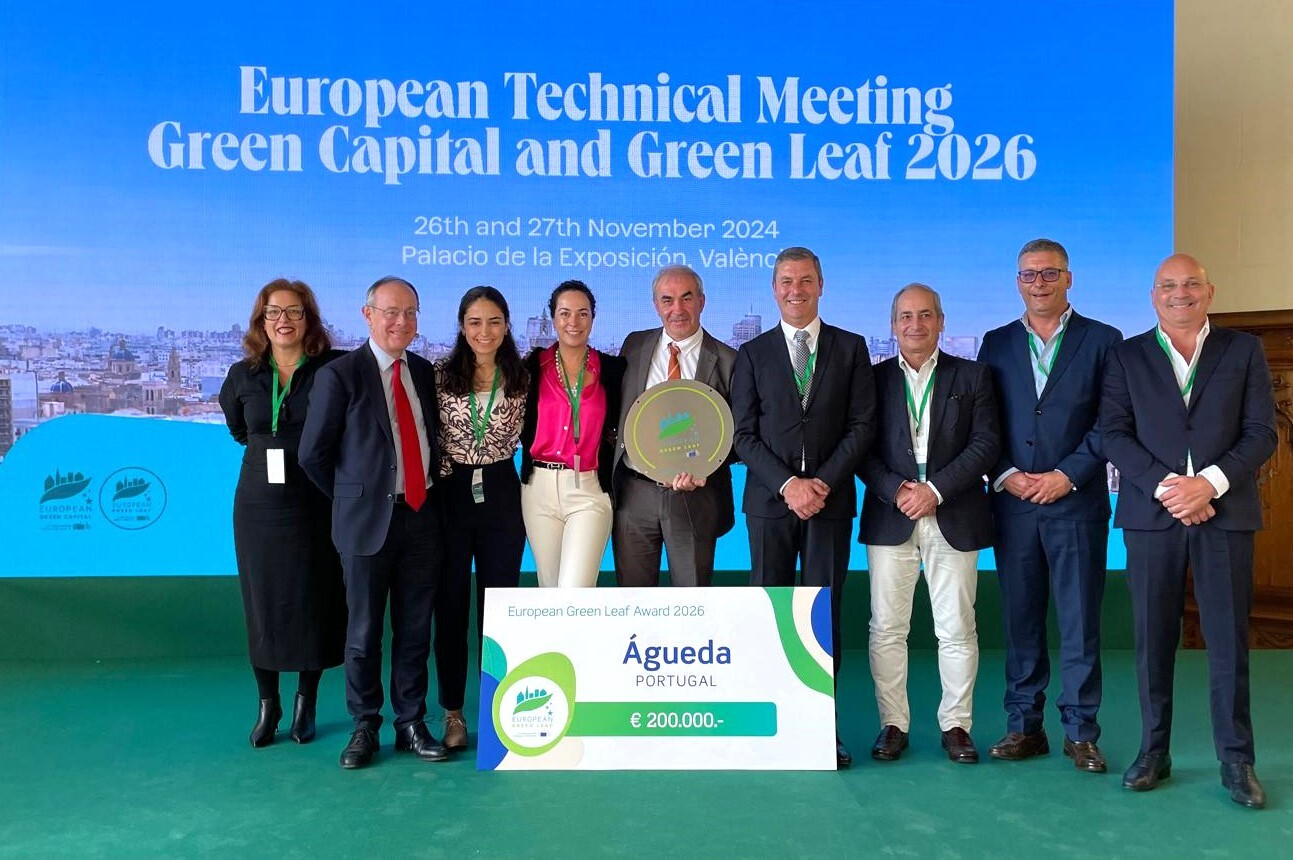
\includegraphics[width=1.15\textwidth]{figures/greenleaf_1_2500_2500.jpeg}
    \caption{Serviço de mobilidade sustentável no Município de Águeda, Portugal, citado na página do município: \cite{Águeda_vence_prémio_European_Green_Leaf_2026}.}
    \label{fig:beaguedapremio}\end{figure}


%%%%%%%%%%%%%%%%%%%%%%%%%%%%%%%%%%%%%%%%%%%%%%%%%%%%%%%%%%%%%%%%%%%%%%%%%%%%%%%%
\section{Polónia: Interação com \textit{Stakeholders}}
\label{sec:polonia_interacao_stakeholders}
O artigo VII, aborda a interação com os \textit{stakeholders} da logística urbana como um fator crucial para o desenvolvimento das cidades no caminho para se tornarem cidades inteligentes, semelhante ao artigo anterior onde predomina a cooperação com toda a comunidade e importância da participação ativa dos \textit{stakeholders}\cite{en15114103} .
Este artigo estuda 280 cidades da Polónia e a pergunta que abordam inicialmente é "Será que as cidades incluem logística nas suas estratégias de desenvolvimento urbano ?" \cite{en15114103}.
A base de cidades inteligentes de acordo com o artigo VII é a cooperação entre as pessoas, logística otimizada, qualidade de vida, economia e tecnologia.

Após a análise destas cidades foi recolhida a informação de que >75\% das cidades estava ausente desta cooperação com os \textit{stakeholders}, pois 85\% da economia das mesmas estava em um circuito fechado, chamado \textit{vendor lock-in} \cite{en15114103}.

\textbf{De notar que:} métricas como nível de adesão dos stakeholders, percentagem de cidades com planos logísticos por partes interessadas e grau de cooperação, são essenciais para dados históricos que permitam avaliar o progresso rumo a cidades inteligentes \cite{en15114103}.

A \gls{fig}: \ref{fig:polonia_interacao_stakeholders},  abaixo demonstra uma análise mais detalhada de províncias da Polónia que foram estudadas no artigo VII \cite{en15114103}.
\begin{figure}[H]
    \centering
    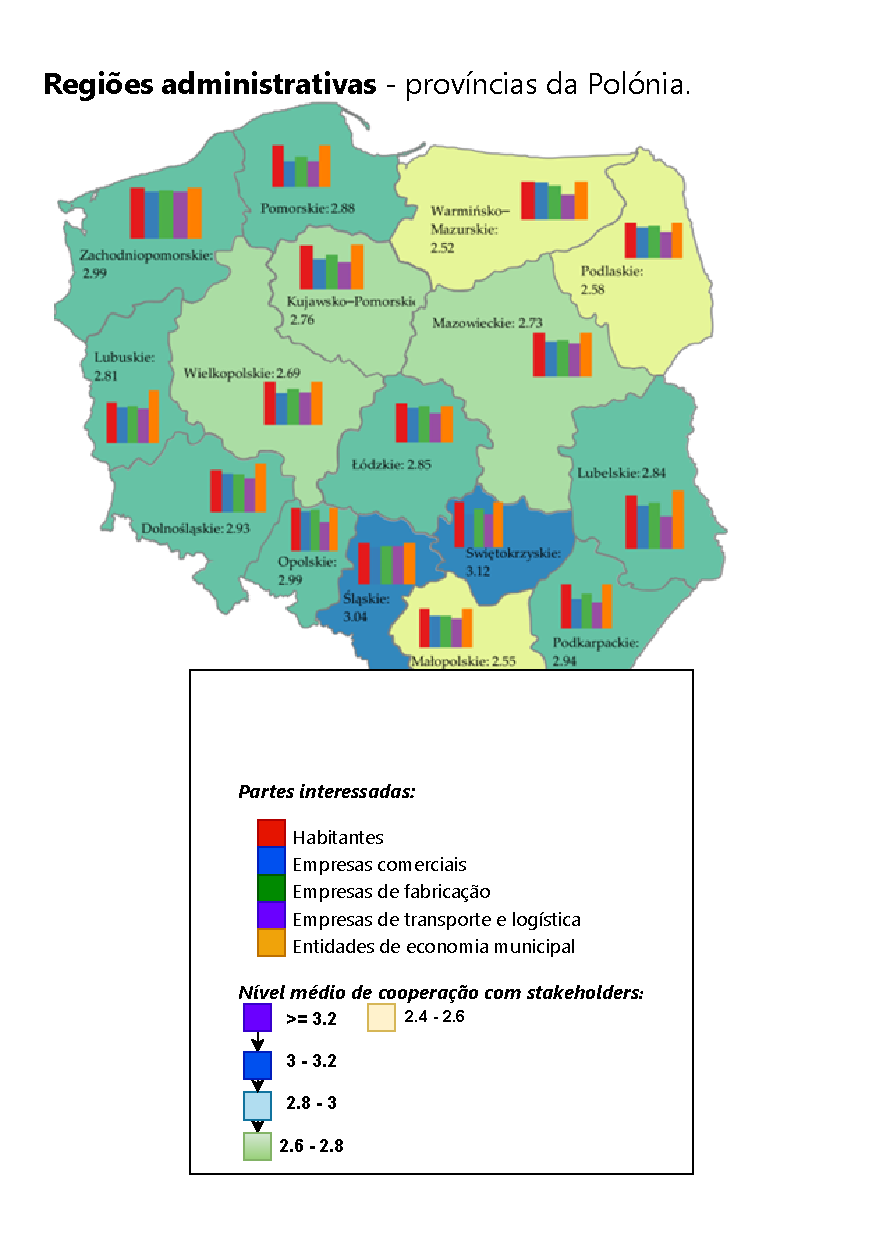
\includegraphics[width=1.0\textwidth]{figures/article7.drawio.pdf}
    \caption{Análise detalhada de províncias da Polónia \cite{JunqueiraDevEduardoRepositório}.}
    \label{fig:polonia_interacao_stakeholders}
\end{figure}
Asim, podemos concluir que a verdadeira inteligência de uma cidade urbana vem de um bom planeamento lógico, cooperação entre todos os \textit{stakeholders} e implementação de normas globais \cite{en15114103}.
%%%%%%%%%%%%%%%%%%%%%%%%%%%%%%%%%%%%%%%%%%%%%%%%%%%%%%%%%%%%%%%%%%%%%%%%%%%%%%%
%Revisto tudo!